%\begin{savequote}[8cm]
%Simplicity is prerequisite for reliability.
%  \qauthor{--- Edsger W. Dijkstra}
%\end{savequote}

\chapter{An introduction to modular assembly}
\label{ch:polycubes_intro}

\minitoc

This chapter will provide a background on modular self--assembly, starting with an explanation of how nucleic acids can be used as a building material and followed by examples of experimentally realised multicomponent structures. The final section will cover relevant self--assembly theory, presenting tile assembly models and their results.

%Components that self--assemble into such chrystals can also assemble bounded structures, if only a way can be found to make them self--limiting. 

\section{Nucleic acids as a building material}
Professor Ned Seeman was inspired to pioneer the field of \emph{structural DNA nanotechnology} after seeing the woodcut \emph{Depth} by M.C. Escher, where fish are depicted organised into a crystalline structure \cite{seeman_2016}. As it turned out, the nucleic acid strands of DNA (and later also RNA) could be designed to self--assemble into similar structures if the strand sequences were chosen cleverly enough, as this section will explain.

\subsection{DNA structures}

The main building material covered in this thesis is deoxyribonucleic acid (DNA). DNA is a linear polymer more known for encoding the genes of living systems \cite{calladine1997understanding}. Strands of DNA are made up of units called \emph{nucleotides}, consisting of a sugar--phosphate backbone unit, as well as one of four possible bases: \emph{adenine} (\textbf{A}), \emph{thymine} (\textbf{T}) \emph{cytosine} (\textbf{C}), and \emph{guanine} (\textbf{G}). 

Two strands of DNA can bind together to form a helical duplex. Through Watson--Crick base--pairing, the \textbf{A} nucleotide form two hydrogen bonds with \textbf{T}, while \textbf{G} forms three with \textbf{C}, making DNA double--stranded. Each strand has a directionality, conventionally represented as going from the 3' to the 5' end of the strand, making the duplex anti--parallel.

The base part of the nucleotide is hydrophobic, while the sugar--phosphate backbone is hydrophilic, which means that the bases ``hide'' on the inside of the duplex to avoid contact with water molecules. However, the length of a backbone unit is about 6~Å (0.6~nm), while the bases would need to be at a distance of 3.3~Å (the Van der Waals contact separation) to stack stably (without any room for water) \cite{calladine1997understanding}. To reconcile this inequality, the DNA duplex forms a double--helical structure with a radius of about 9~Å.

While an unbranched double--helix is the most natural confirmation, it is still possible for duplicates to branch into multiple junctions. For example, the Holliday junction is a junction between four double--helical arms, shown in Figure~\ref{fig:holliday} in one of its possible configurations.

\begin{figure}
    \centering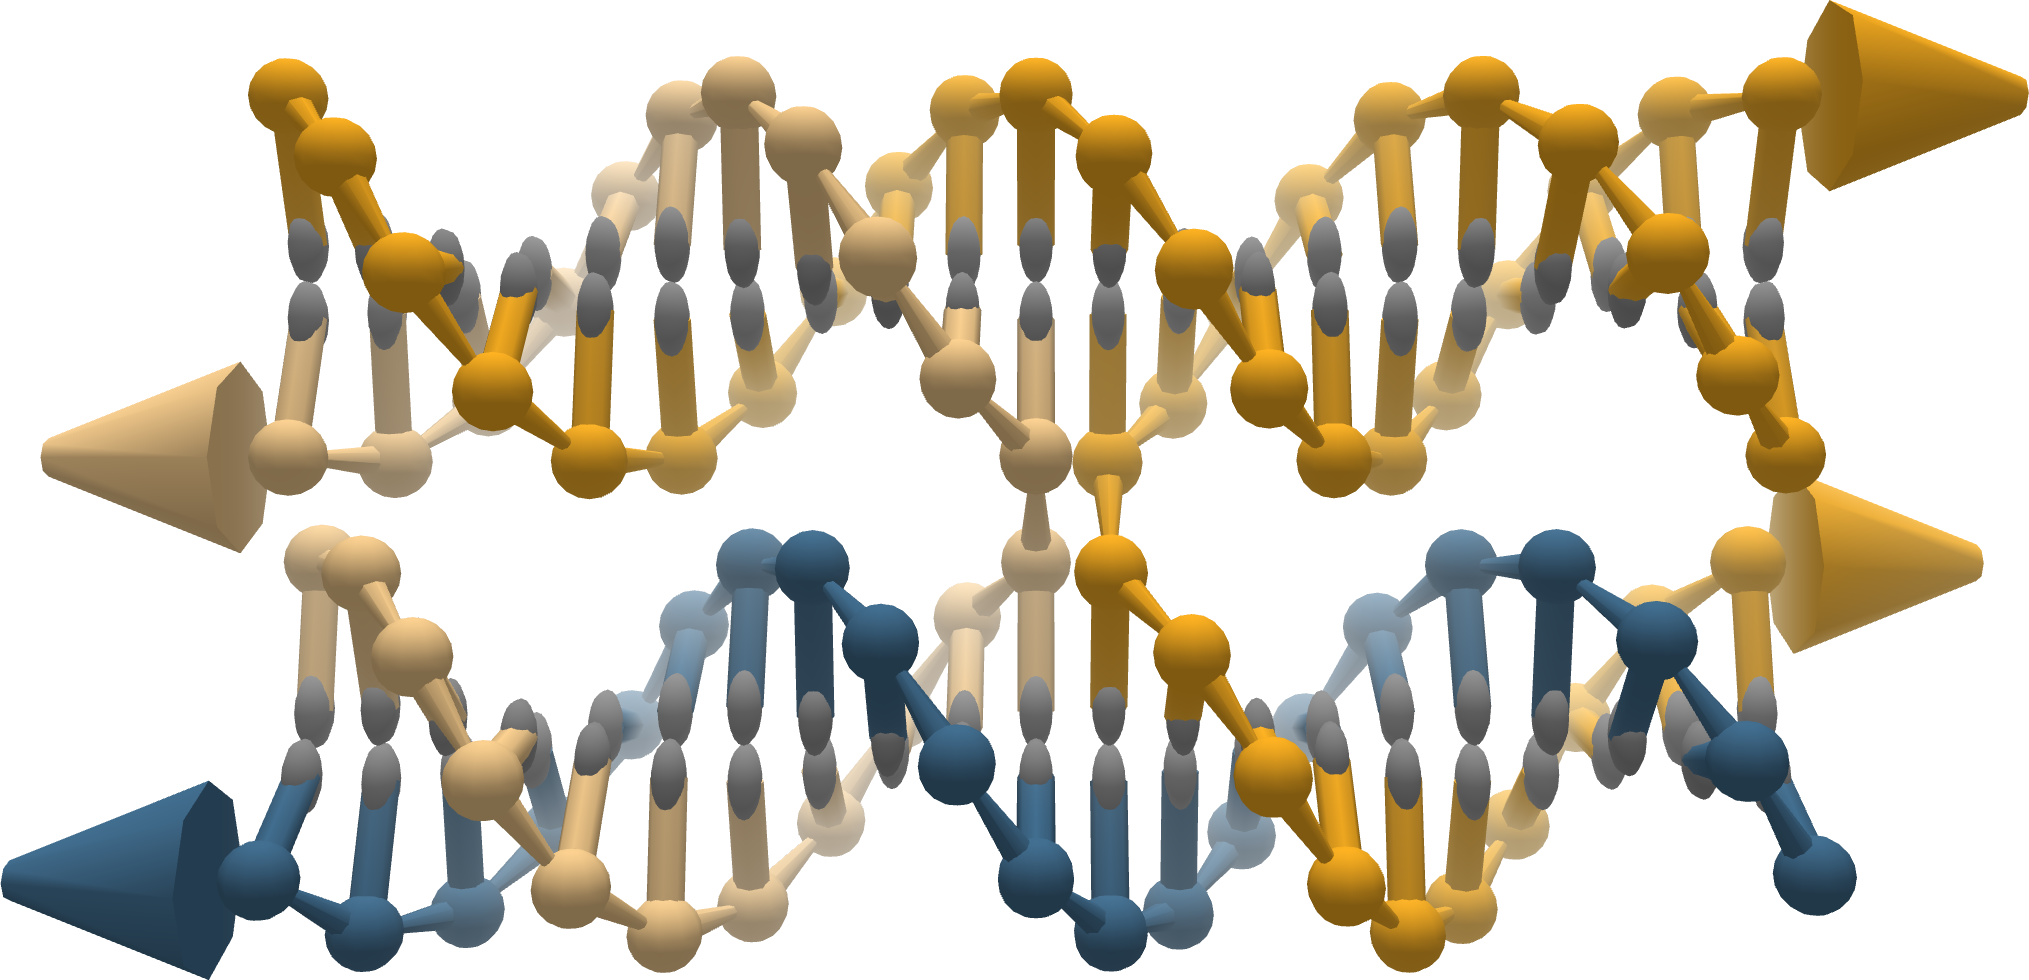
\includegraphics[width=\textwidth]{figures/holliday.png}
    \caption{Holliday junction, designed in oxView. Sugar--phosphate backbone unit are represented as spheres, while bases are represented as gray spheroids (here without any visual distinction between base types). Arrow heads at the end indicate the 3' end of each of the four strands.}
    \label{fig:holliday}
\end{figure}

%https://www.rcsb.org/structure/1M6G

%Double--stranded DNA has a persistence length of approximately [], while single--stranded sections are much more flexible,

By designing sequences with complementary domains corresponding to intended duplex regions, it is possible to create many different DNA motifs and structures \cite{seeman_2016, Seeman1982}, an understanding that pioneered the field of structural DNA nanotechnology and the use of DNA as a building material.

%% Add more here

Another breakthrough in the field was the DNA origami technique \cite{rothemund2006folding}, a now popular and proven method for creating larger irregular structures using DNA. The principle behind it, as illustrated in Figure~\ref{fig:dnaOrigami}, is to use short staple strands, each with one or more domans that are complementary to domains on a viral scaffold strand. As the temperature is gradually lowered, the staples bind to the scaffold as seen in Figure~\ref{fig:dnaOrigami}. If done correctly, this ``folds'' the scaffold into the desired structure, hence the name ``origami''. However, care must be taken to how the scaffold should be routed through the design to avoid kinetic traps where the folding cannot be completed.

With improved design software, it is becoming easier to design DNA origami structures of any given form. See Section~\ref{sec:design_tools} for an introduction to such tools.

% Andrew: I suggest a more extensive discussion of the basis of origami design to accompany an improved/alternate fig:{dnaOrigami}

% Some more added

\begin{figure}
    \centering
    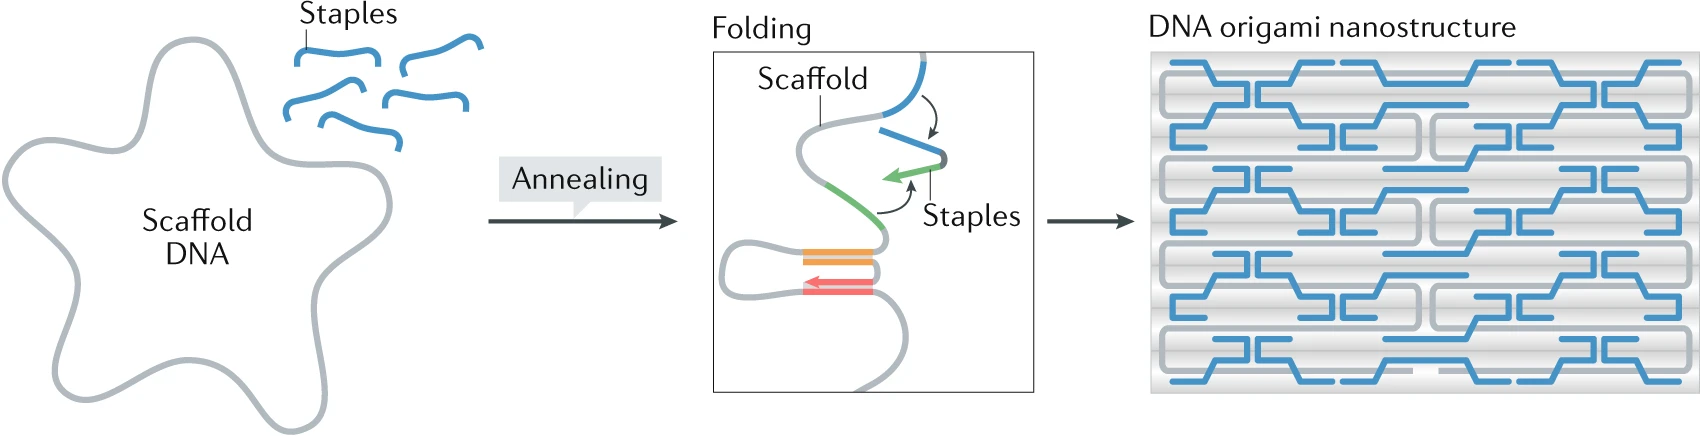
\includegraphics[width=\textwidth]{figures/dna_origami.png}
    \caption{Illustration of \emph{DNA origami} \cite{rothemund2006folding}, adapted from \cite{dey2021dna}. A long scaffold strand, obtained from a virus, is folded into the desired nanostructure by multiple short staple strands binding to complementary domains of the scaffold.
    }
    \label{fig:dnaOrigami}
\end{figure}

In DNA origami, the size of the structure is limited by the length of the scaffold, which motivates researchers to investigate approaches with multiple origami modules. Some previous results will be described in Section~\ref{sec:experimental_appl}. The work described in this thesis aims to simplify the design process significantly.

\subsection{RNA structures}
\label{sec:RNA_design}
Another promising building material for self--assembly is ribonucleic acid (RNA). RNA is very similar to DNA, but with a backbone containing the sugar ribose, instead of the deoxyribose sugar found in DNA, and with the \emph{thymine} base (\textbf{T}) replaced by \emph{uracil} (\textbf{U}).

Biologically, DNA is transcribed into RNA by the RNA polymerase enzyme as part of gene expression \cite{sadava2014life}. While DNA folding is easier to predict, the more reactive RNA backbone offers the possibility of a more functionalised structure; for example, by incorporating aptamers, enzymes, and other such modifications \cite{guo2010emerging}.

% TODO from Andrew: Check the above paragraph

In 2014, Geary et al., from the Andersen lab in Aarhus, demonstrated a method \cite{geary2014single, sparvath2017computer, geary2021rna} for co--transcriptionally folded RNA origami, which also enables folding \emph{in vivo}. As shown in Figure~\ref{fig:rna_origami}, the design used a set of tertiary RNA motifs (such as kissing hairpins and double crossovers) as modules. These modules are combined to generate a blueprint for a single strand, enforcing the desired self--interactions. Finally, an iterative algorithm is used to find a sequence that should co--transcriptionally fold into the intended shape.

\begin{figure}[h]
  \centering
  \begin{overpic}[width=\textwidth]{figures/rna_origami.png}
      \put(0,600){a)}
      \put(0,250){b)}
      \put(0,110){c)}
      \put(510,600){d)}
      \put(510,430){e)}
      \put(510,310){f)}
      \put(510,150){g)}
  \end{overpic}
  \caption{Co--transcriptional folding of RNA origami, adapted from \cite{geary2021rna}. \textbf{a)} The set of RNA motifs used as modular building blocks. \textbf{b)} Schematic of the modules connected to form a single strand. \textbf{c)} Atomistic model of the design in b). \textbf{d)} Shows the text--based blueprint used to create designs, while \textbf{e)}, \textbf{f)}, and \textbf{g)} shows scripts developed to aid the visualisation and preform sequence design for the origami.}
  \label{fig:rna_origami}
\end{figure}

The Andersen lab is one of the partners of the ITN network I am part of, and I have spent a two--month secondment there working with their RNA origami method. Some of my results on simulating RNA designs are covered in Section~\ref{sec:converting_rna_origami}.

% Andrew: A description of how RNA design is different (different helical structure & why it matters, single--stranded vs. multiple strands)

% "The emerging field of RNA nanotechnology might seem more promising in this regard because RNA is readily transcribed into a single strand in cells, which can be directly folded into a programmed nanostructure"
% https://www.nature.com/articles/nnano.2011.187


\section{Examples of modular nucleic acid structures} \label{sec:experimental_appl}
From small tiles made from a handful of strands to megadalton--scale structures made from multiple origami designs, modular self--assembly has seen considerable experimental research. This section provides a quick overview of some results of particular interest to the polycube model presented in Chapter~\ref{ch:polycubes1}.


\subsection{DNA tiles}
\label{sec:dna_tiles_bricks}
Following early nucleic acid multi--arm junctions and lattices suggested by Seeman \cite{seeman1982nucleic}, Winfree \cite{winfree1998algorithmic, winfree1998design} used double--crossover (DX) motifs, shown in Figure~\ref{fig:dna_tiles}.a, to self--assemble 2D DNA crystals. 
% Andrew: Describe how 4 sticky ends govern ?sossably?
The tiles attach using so--called \emph{sticky ends} where, as seen in Figure~\ref{fig:dna_tiles}.a, one of the strands continue past the end of a duplex region. Each tile has four such sticky ends, so it can can connect to four other tiles (as seen in Figure~\ref{fig:dna_tiles}.b) if their respective sticky end regions have complementary sequences. Also seen in Figure~\ref{fig:dna_tiles}.b, the lattices could be made with varying complexity, exemplified using either two or four different species of tiles.
% Tiles: https://www.nature.com/articles/28998

\begin{figure}[h]
  \centering
  \begin{overpic}[width=0.7\textwidth]{figures/dna_tiles.png}
    \put(0,450){a)}
    \put(0,240){b)}
  \end{overpic}
  \caption{DX tiles forming 2D lattices, adapted from \cite{winfree1998design}. \textbf{a)} Examples of tile designs with double--crossover motifs. \textbf{b)} Lattices made using two and four tile species respectively.}
  \label{fig:dna_tiles}
\end{figure}

\subsection{RNA tiles}

% Andrew: Other RNA structures?

%https://www.science.org/doi/abs/10.1126/science.1253920 
As already covered in Section~\ref{sec:RNA_design}, it is possible to co--transcriptionally fold \emph{RNA origami} \cite{geary2014single}. This was first shown in 2014 by Geary et al., who folded RNA tiles that connect through complementary 120-degree kissing loop interactions, as seen in Figure~\ref{fig:rna_tiles}, forming a hexagonal lattice. A significant promise with co--transcriptionally folded RNA structures is that they can be assembled \emph{in vivo} \cite{guo2010emerging}, with a DNA gene being transcribed into RNA inside a cell.

\begin{figure}[h]
  \centering
  \begin{overpic}[width=\textwidth]{figures/rna_tiles.jpeg}
      \put(0,300){a)}
      \put(320,300){b)}
      \put(750,300){c)}
  \end{overpic}
  \caption{Co--transcriptional folding RNA origami tiles, adapted from \cite{geary2014single}. The tiles connect through 120-degree kissing loop interactions, forming a hexagonal lattice. \textbf{a)} Detailed scematic of the four--helix 4H--AO tile. \textbf{b)} Co--transcriptional folding, where the RNA tile folds as it is transcribed from a DNA template. \textbf{c)} Hexagonal lattice formed by folded tiles.}
  \label{fig:rna_tiles}
\end{figure}

\subsection{DNA bricks}
% Bricks: https://www.nature.com/articles/nature24648

A three--dimensional DNA ``canvas'' was created in 2017 by Ong et al. \cite{ong2017programmable}, using a technique called \emph{DNA bricks}. Structures were assembled from up to about 30,000 unique components, as seen in Figure~\ref{fig:dna_bricks}. 
Each ``brick'' component consists of a single, 52 nucleotides long, DNA strand. The strand has four 13-nucleotide domains, each complementary domains to a domain in a neigbouring brick. A 13-nucleotide helix corresponds to approximately 1.25 turns, creating a 90$^{\circ}$ dihedral angle between the bricks, as Figure~\ref{fig:dna_bricks}.a shows.

Since each brick is unique, custom shapes can be ``sculpted'' by leaving out the voxels (3D pixels) not required.



% Andrew: Again, a missed opportunity to describe what is going on (4x8-base domains - interactions with neighbours - helical repeat)


\begin{figure}[h]
  \centering
  \begin{overpic}[width=\textwidth]{figures/dna_bricks.png}
    \put(0,350){a)}
    \put(450,350){b)}
    \put(450,120){c)}
  \end{overpic}
  \caption{DNA bricks, adapted from \cite{ong2017programmable}. \textbf{a)} DNA brick structure, where each of the up to 30'000 unique components is a 52 nucleotide DNA strand. The strands connect through a 13 base pair complementary domain at a 90 degree dihedral angle. \textbf{b)} A cuboid, here shown with 10,000 components, corresponds to a 20,000 voxel canvas. \textbf{c)} Approximating the shape of a teddy bear by removing a subset of the voxels from the canvas.}
  \label{fig:dna_bricks}
\end{figure}

\subsection{Finite DNA origami arrays}
\label{sec:origamiArrays}
% https://www.nature.com/articles/nature24655

In 2017, Tikhomirov et al. \cite{tikhomirov2017fractal, tikhomirov2017programmable} used the DNA origami technique to demonstrate two--dimensional patterns assembled on the micrometre--scale using square tiles where each tile was a complete origami, as seen in Figure~\ref{fig:origamiArrays}. The tiles connect to each other through complementary single--stranded overhangs on their edges.

The patterns could either be hierarchically assembled from unique tiles \cite{tikhomirov2017fractal} or assembled into random patterns from a small number of tile types \cite{tikhomirov2017programmable}. The binding strength could be adjusted using a variable amount of edge overhangs, as seen in Figure~\ref{fig:origamiArrays}.b). Arrays up to \(8 \times 8\) tiles were successfully produced, although larger arrays had a much smaller yield (Figure~\ref{fig:origamiArrays}.c).

While the random tilings were generally unbounded, Tikhomirov et al. also showed how to program a finite grid, as seen in Figure~\ref{fig:origamiArrays}.d). These tiles are very similar to the polyomino model later described in Section~\ref{sec:polyomino}.

\begin{figure}[h]
  \centering
  \begin{overpic}[width=\textwidth]{figures/monalisa_tiles.png}
    \put(-20,580){a)}
    \put(200,580){b)}
    \put(-20,150){c)}
    \put(600,580){d)}
  \end{overpic}
  \caption{DNA origami arrays, adapted from \cite{tikhomirov2017fractal, tikhomirov2017programmable}. \textbf{a)} Strand--level diagram of a \(12 \times 12\) version of the the origami tile (actual size is \(22 \times 22\) helices). \textbf{b)} \(4 \times 4\) tile ``Mona Lisa'' pattern. The pattern is achieved through double--stranded extensions of selected staple strands inside each origami tile. Staples with the extension correspond to pixels turned on, while those without are turned off. \textbf{c)} AFM image of patterned assemblies of different sizes (left) with their respective yields (right). \textbf{d)} Abstract design diagrams (left) and AFM images (right) of finite origami arrays, designed to different sizes \cite{tikhomirov2017programmable}.}
  \label{fig:origamiArrays}
\end{figure}

\subsection{Shape--complementary origami}
\label{sec:shape-complementary}
% 2D https://www.nature.com/articles/nchem.1070
% 3D https://science.sciencemag.org/content/347/6229/1446.abstract

% Huge https://www.nature.com/articles/s41563-021-01020-4

Also in 2017, Wagenbauer et al. \cite{wagenbauer2017gigadalton} used shape--complementarity to assemble DNA origami components into three--dimensional polyhedral shapes up to 450 nanometers in diameter. Later, in 2021, Sigl et al. assembled large shells from shape--complementary origami triangles, as seen in Figure~\ref{fig:shape-complementarity}. The triangular sides attach through protrusions and indentations of complementary shape, as seen in Figure~\ref{fig:shape-complementarity}.a). By having extra helices protruding from one triangle side, and a hole with a shape they would fit on the side of another triangle, the two components can binding together through stacking interactions at the helix ends, a method first shown by Woo et al. \cite{woo2011programmable}.

While the described experiments use triangular components, the general shape--complementary assembly method is a relevant option for a physical realization of the torsionally rigid polycube patches described in Chapter~\ref{ch:polycubes1}.

\begin{figure}[h]
  \centering
  \begin{overpic}[width=\textwidth]{figures/icosahedral_shell.png}
    \put(0,320){a)}
    \put(620,320){b)}
  \end{overpic}
  \caption{Shape--complementary triangles assembling polyhedral shells. Adapted from \cite{sigl2021programmable}. \textbf{a)} Polyhedral shell design for T=9. \(N\) is the triangulation number (the number of unique edges required for assembly), \(\alpha\) is the bevel angle of the triangle sides, and \(N\) is the number of triangles required for a full shell. \textbf{b)} Cryo--EM reconstruction of an assembled T=4 icosahedral shell.}
  \label{fig:shape-complementarity}
\end{figure}


\subsection{DNA origami nanochambers}
% https://pubs.acs.org/doi/full/10.1021/jacs.0c07263

In 2020, Lin et al.\cite{nano-chambers_lin2020} presented cubic DNA origami ``nanochambers''. The chambers have sticky--end overhangs on every side of the cube, allowing it to assemble in one, two and three dimensions, as can be seen in Figure~\ref{fig:nanochambers}. However, since the shape is only rotationally symmetric around the z--axis, the assembly is a still only a limited subset of the polycube model described in Chapter~\ref{ch:polycubes1}. 

\begin{figure}[h!]
  \centering
  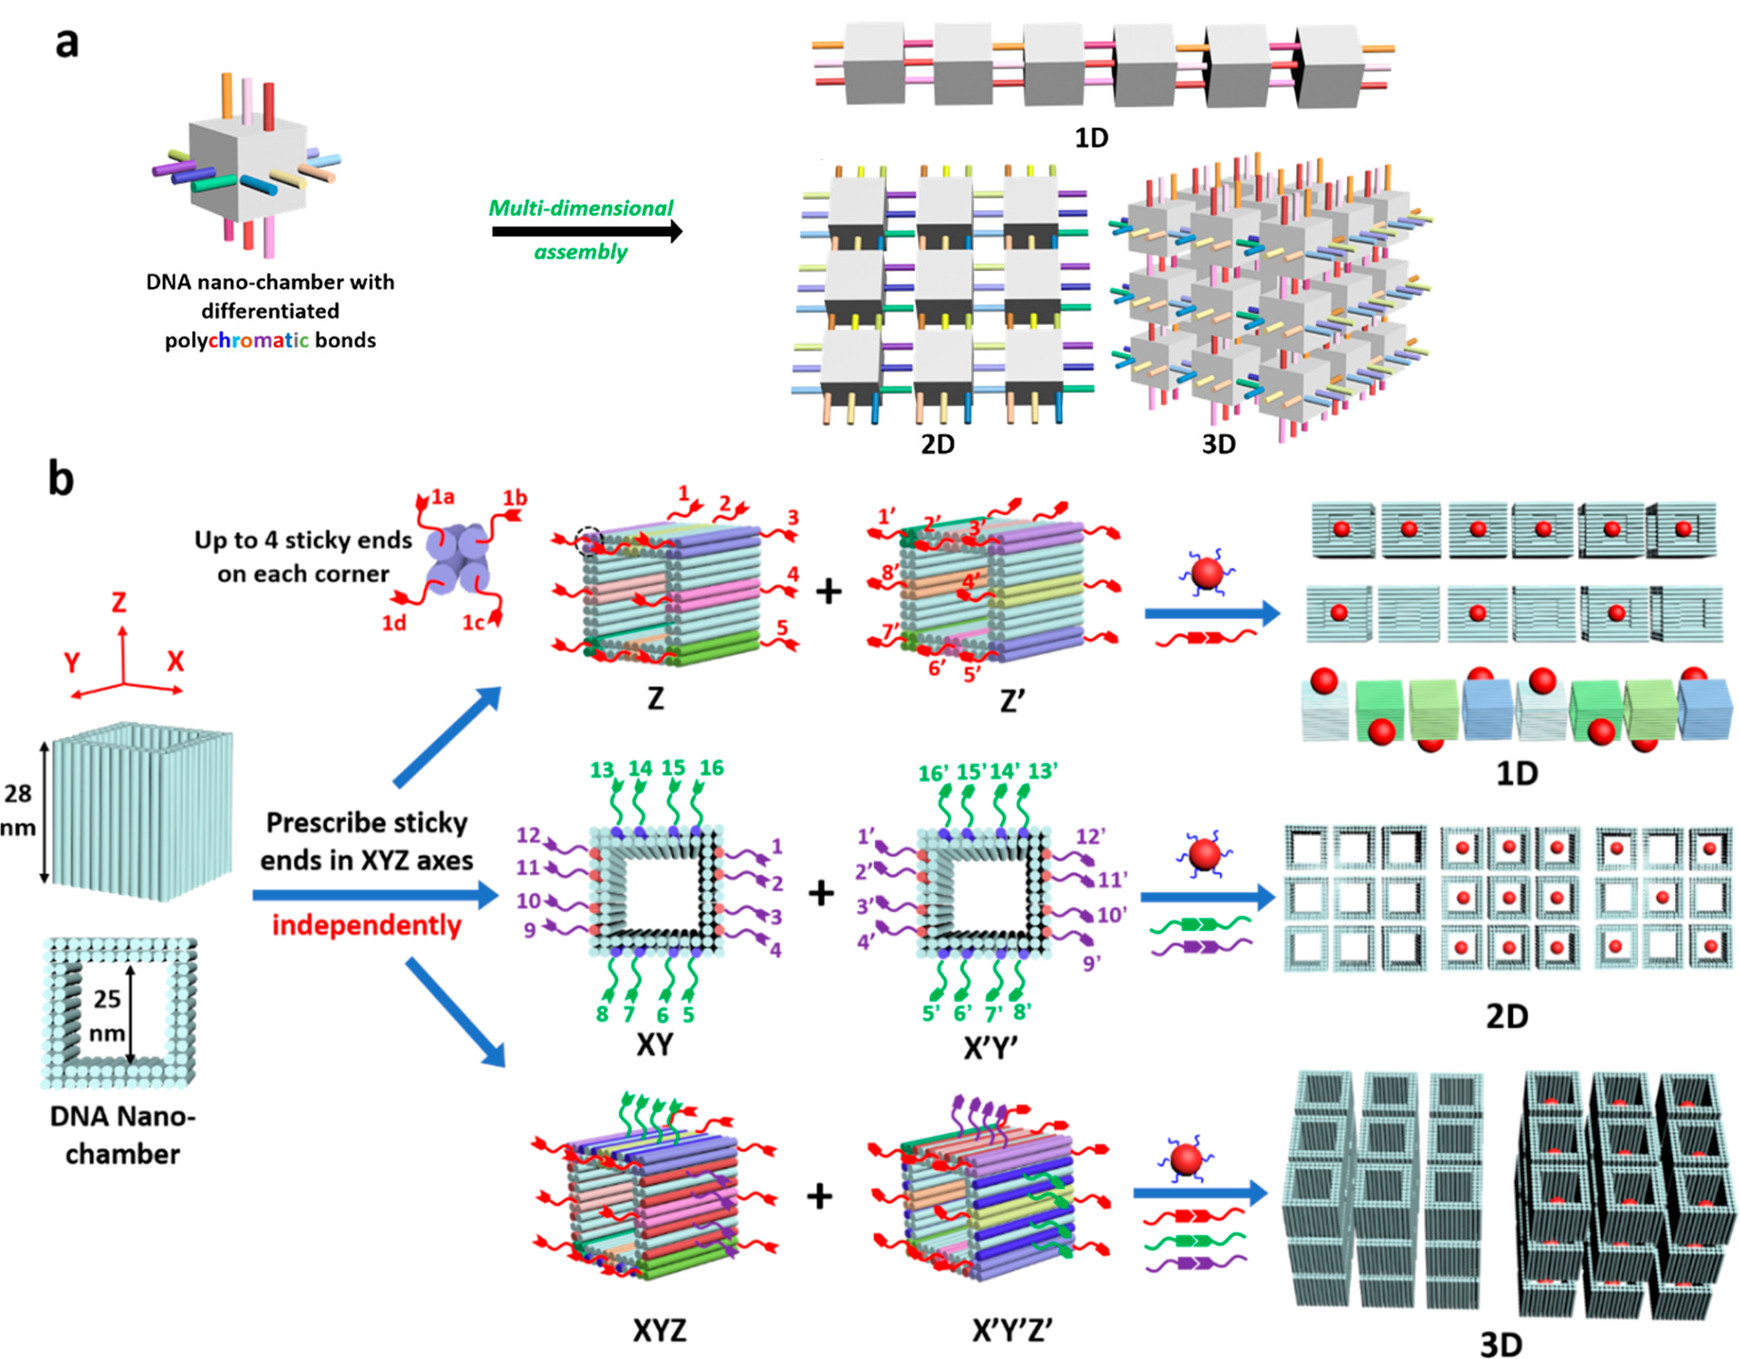
\includegraphics{figures/nanochambers2.jpeg}
  \caption{DNA origami nanochambers, adapted from \cite{nano-chambers_lin2020}. \textbf{a)} Concept illustration, where building blocks with \emph{polychromatic} bonds (differentiated though different single--stranded sequences), assemble into 1D, 2D, and 3D structures. \textbf{b)} Schematic of DNA nanochamber programmable assembly, showing sticky end overhangs applied in 1D, 2D, and 3D assemblies.}
  \label{fig:nanochambers}
\end{figure}

\subsection{Octahedral DNA origami frames}
In 2020, Wang et al. \cite{tian_octahedra2020} showed how octahedral DNA origami frames could be used as building blocks in limited and unlimited programmed assemblies, as seen in Figure~\ref{fig:tian_octahedra}. Using sticky--end overhangs at the octahedral vertices, the building blocks have the connectivity, as well as the rotational symmetry, of a cube.

Due to the flexibility of the single--stranded connections, the connections are less torsionally rigid than assumed in the polycube model, later described in Chapter~\ref{ch:polycubes1}. However, as can be seen in Figure~\ref{fig:tian_octahedra}, shapes such as the cube can still be assembled with good yield.

% https://onlinelibrary.wiley.com/doi/abs/10.1002/anie.201913958

\begin{figure}[!h]
  \centering
  \begin{overpic}[width=\textwidth]{figures/tian.jpg}
    \put(0,480){a)}
    \put(280,480){b)}
    \put(670,480){c)}
  \end{overpic}
  \caption{Octahedral DNA origami frames, adapted from \cite{tian_octahedra2020}. \textbf{a)} Two octahedra with complementary sticky ends binding together to form a dimer. The edges consist of six--helix bundles. \textbf{b)} nanoclusters assembled from different sets of building blocks. \textbf{c)} \(2 \times 2 \times 2 \) cube nano cluster (top) and histogram of the mass fraction, where the intended design of eight components per cluster is the most common.}
  \label{fig:tian_octahedra}
\end{figure}


\FloatBarrier
\section{Theory of modular self--assembly}

With some experimental background covered, let us now look at the progress on the theoretical side of self--assembly design. Although the designs covered are built from nucleic acid strands, it would be computationally impractical to include that level of detail in a self--assembly model. A more straightforward approach is instead to model each component as a discrete tile on a lattice. This section will present earlier such models as a background to my own polycube model, which will be introduced in Chapter~\ref{ch:polycubes1}.

For all modular designs, an important factor is the number of unique components needed. This relates to the concept of complexity covered in Section~\ref{sec:AIT}.

\subsection{Wang tiles}
Introduced by Hao Wang in 1961 \cite{wang1961proving}, \emph{Wang tiles} are square tiles with a colour assigned to each of their four edges. Without rotating or reflecting the tiles, they assemble so that adjacent edges have the same colour.

%\begin{figure}[h]
 % \centering\includesvg[width=0.5\textwidth]{figures/Wang_11_tiles.svg}
 % \caption{Wang tiles}on
%\end{figure}

The DNA tiles by Winfree et al. \cite{winfree1998design}, presented in Section~\ref{sec:dna_tiles_bricks}, behave like Wang tiles by design and do not allow rotations or reflections. Winfree investigated the possibility of using such tiles for computation \cite{winfree1998algorithmic}, which led to aTAM: the algorithmic Tile Assembly Model.

\subsection{The algorithmic tile assembly model}
\label{sec:atam}
% David Doty overview: https://cacm.acm.org/magazines/2012/12/157881-theory-of-algorithmic-self-assembly/fulltext

% Molecular algorithms https://www.nature.com/articles/s41586-019-1014-9

The algorithmic Tile Assembly Model (aTAM), shown in Figure~\ref{fig:atam}, models the dynamic behaviour of the double crossover DNA tiles introduced by Winfree et al. \cite{winfree1998design}. Each tile has four patches, one on each edge, corresponding to the four sticky ends of the DNA tile. Furthermore, the patches can have different strengths, with a global temperature variable determining the total connection strength required for a tile to attach \cite{doty2012theory}.

In the example seen in Figure~\ref{fig:atam}, the pattern grows from the initial bottom--right seed into the blue horizontal bottom row and the rightmost vertical column. This is because these tiles have ``strength-2'' glues with enough binding strength to attach by themselves \cite{doty2012theory}. The additional tiles have weaker ``strength-1'' glues (illustrated as thinner black connectors), so they need at least two complementary patches to achieve the binding strength threshold (temperature).

Because of this so--called \emph{co--operative binding}, the tiles can be seen as logic gates performing computation; given the bottom and right patches as input bits, the matching tile attaches and produces two computed output bits (top and left).

% Ard: You should mention that a key interest in this model is because it is thought to be Turing universal.


\begin{figure}[h]
  \centering\includesvg[width=\textwidth]{figures/atam.svg}
  \caption{Algorithmic self--assembly of a Sierpiński triangle. Adapted from \cite{doty2017}. A tile set (right) grows from an initial seed by co--operatively attaching self--complementary edges (without rotation). The \(0\) and \(0\) ``glues'' are weaker and require two matching bonds to attach (co--operative binding), compared to the \(W\) (west) and \(N\) (north) glues that are strong enough to bind alone.}
  \label{fig:atam}
\end{figure}

\subsection{The polyomino model}\label{sec:polyomino}

% Ard: I think you need a longer section on the background of the polyomino model here. This is very terse.

The main inspiration for the \emph{polycube} model (presented in Chapter~\ref{ch:polycubes1}) is the polyomino model \cite{ahnert2010self, johnston2011evolutionary}. As noted in Section~\ref{sec:origamiArrays}, the 2D model is similar in assembly to the later experimental micrometer scale tile designs by Tikhomirov \cite{tikhomirov2017programmable} shown in Figure~\ref{fig:origamiArrays}.d). Compared to the aTAM model described in Section~\ref{sec:atam}, polyomino tiles are allowed to rotate (but not invert), creating further possibilities for symmetries. Also, the edge binding is not self--complementary, with complementary colour pairs used instead. Finally, polyominoes have a constant binding strength, assembling irreversibly and without co--operative binding (corresponding to ``strength-0'' glues).

See Figure~\ref{fig:polyominoes} for an illustration of the model, where an input \emph{genotype} (describing the four possible tile types) is mapped into an assembled output polyomino phenotype by stochastically growing the shape from an initial seed. The growth stops if, as in the figure, no more tiles can attach (since the colour \(0\) does not bind to anything). If the growth is infinite, the genotype is called \emph{unbounded}. A genotype is considered \emph{deterministic} if it assembles the same phenotype polyomino every time. Only output corresponding to bounded and deterministic genotypes are considered valid.

\begin{figure}[h]
    \centering
    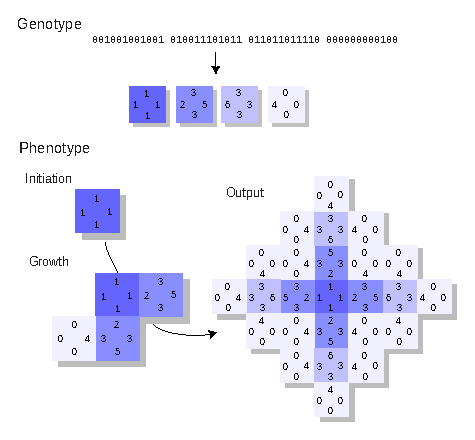
\includegraphics[width=0.6\textwidth]{figures/polyominoes.eps}
    \caption{Illustration of the polyomino assembly model, adapted from \cite{johnston2011evolutionary}. A \emph{genotype}, in the form of a ruleset of possible tiles, encodes for a polyomino \emph{phenotype}, grown stochastically from an initial seed tile. The integers on the tile edges represent the colour of that edge, where every even integer \(n\) binds to the odd \(n-1\). The exception is tile edges with the colour \(0\) that does not bind at all. The output phenotype is grown from an initial seed, a tile of the first species defined in the genotype. Additional tiles, from any species in the genotype, are then added wherever there are compatible edge colours.}
    \label{fig:polyominoes}
\end{figure}

\subsection{Algorithmic Information Theory and input-output maps}
\label{sec:AIT}
% https://www.ox.ac.uk/news/science-blog/%E2%80%98simplicity-bias%E2%80%99-science

% https://www.nature.com/articles/s41467-018-03101-6

% https://solo.bodleian.ox.ac.uk/permalink/f/89vilt/oxfaleph022417805

%Some things, whether in the form of a shape, a song, or a binary string, require less information to describe than others.

If we have a self--assembly model mapping from an input set of building blocks into an output shape, can we find the simplest input for a given output? To answer this, we first need to consider what we mean by ``simplest''; what is the \emph{complexity} of a shape?

Complexity has different definitions in different fields, but here we focus on the amount of information needed to describe something, in this case, a shape. Some things, whether in the form of a shape, a song, or a binary string, clearly require less information to describe than others, and we would then call those less complex than their counterparts, but how can we quantify that difference?

Let us first consider the complexity of text strings. If you have a monkey pressing random keys on a typewriter, you would expect it to produce every string of length \(N\) with equal probability (assuming the keystrokes were indeed truly random). With \(k\) keys on the keyboard, the probability for any string of length \(N\) is then \(k^{-N}\). For example, the title of this thesis, while unlikely to appear randomly, would be equally as probable as any other 50-character string, see the three example strings below, all with probability \(k^{-50}\):
\begin{lstlisting}[numbers=left]
  DESIGN AND MODULAR SELF--ASSEMBLY OF NANOSTRUCTURES
  SHWDRVWKFORWJDOEXOZLSBNREKC Z  VSDJJF  ROKFYRVMIUI
  AAAAAAAAAAAAAAAAAAAAAAAAAAAAAAAAAAAAAAAAAAAAAAAAAA
\end{lstlisting}

But what if we described our strings using algorithms, rather than a full listing of the letters it contains? For example, string number three above could, similarly to the others, then be described using the C programming language as the algorithm:

\begin{lstlisting}[language=c]
printf("AAAAAAAAAAAAAAAAAAAAAAAAAAAAAAAAAAAAAAAAAAAAAAAAAA");
\end{lstlisting}

But now, a much shorter description also exists:

\begin{lstlisting}[language=c]
for(int i=50; i--;) printf("A");
\end{lstlisting}

There are also a number of possible valid variations of the code above, with different variable names and coding conventions, all producing the same output. In other words, not only is the description shorter than writing out the full string but multiple inputs map to the same output, increasing the probability of that particular output further. It also feels intuitive that a string repeating a single letter should be less complex than a random--looking alternative, so this definition of complexity feels reasonable.

The concept of using the shortest possible computer program that can describe an object (for example, a binary string) to determine its complexity is central within the field of Algorithmic Information Theory (AIT) and is called \emph{Kolmogorov complexity} (or Solomonoff–Kolmogorov–Chaitin to give full credit) \cite{LiMing2019AitK}. More specifically, the Kolmogorov complexity \(K(x)\) of an output \(x\) is the length of the shortest program that generates \(x\) on a Universal Turing Machine (UTM) \cite{LiMing2019AitK}.

AIT also includes the \emph{coding theorem}, introducing lower and upper bounds for the probability \(P(x)\) of generating a binary string \(x\) as \(2^{-K(x)} \le P(x) \le 2^{-K(x) + \mathcal{O} (1)}\). In other words, low--complexity outputs are exponentially more likely to be generated by random input compared to high--complexity outputs. This could be compared to how there are many more programs generating the ``simple'' string number three above compared to the randomly generated string two or the carefully selected string one.

However, a problem with Komologrov complexity is that finding the shortest program for a given output is far from trivial (it is, in fact, \emph{uncomputable} in general, due to the \emph{halting problem} \cite{LiMing2019AitK}). Fortunately, Dingle at al \cite{dingle2018input} were able to derive an upper bound to the probability using a computable approximation \(\widetilde{K}(x)\) of the Komologrov complexity:

\[
  P(x) \lesssim 2^{-a\widetilde{K}(x) -b}
\]

The constants \(a\) and \(b\) depend on the input--output map used (but are independent of \(x\)). This is very helpful for calculating the complexity of self--assembled shapes, where properties of the simplest known input rule can be used as such a Komologrov complexity proxy, as will be seen in Section~\ref{sec:polyomino_evolve} and Chapter~\ref{ch:polycubes1}.

\subsection{Evolving polyominoes}
\label{sec:polyomino_evolve}

Evolutionary runs of polyominoes, where a genetic algorithm mutates a genotype population and selects surviving shapes depending on their size, showed a clear bias toward structures with low complexity and high symmetry \cite{johnston2021}. See Figure~\ref{fig:polyomino_symmetries}, where the frequency of protein complexes and polyominoes are compared to their complexity. The number of interface types required (number of patch colours in the polyomino case) is used as a proxy measure for the Komologrov complexity of the structure (see Section~\ref{sec:AIT}).

The evolutionary fitness of the polyominoes only depended on their size (16--mers had the highest fitness), so the simplicity was not selected for but is instead a property of the mapping. This finding is in line with the Algorithmic Information Theory arguments made by Dingle et al. \cite{dingle2018input}, who showed the same simplicity bias for a set of various input--output maps.

\begin{figure}[h]
  \centering
  \begin{overpic}[width=0.9\textwidth]{figures/polyomino_symm_and_simpl.eps}
    \put(0,750){a)}
    \put(520,750){b)}
    \put(0,590){c)}
    \put(520,590){d)}
  \end{overpic}
  \caption{Frequent symmetry and simplicity through evolution, adapted from \cite{johnston2021}. Both protein complexes (a) and polyominoes (b) self--assemble from individual units. \textbf{c)} Frequency of 6--mer protein complex topologies in the protein data bank, versus their complexity (measured as the number of interface types) \textbf{d)} Frequency versus complexity of polyominoes found in evolutionary runs with a fitness function seeking 16--mers.}
  \label{fig:polyomino_symmetries}
\end{figure}
